% Options for packages loaded elsewhere
\PassOptionsToPackage{unicode}{hyperref}
\PassOptionsToPackage{hyphens}{url}
\PassOptionsToPackage{dvipsnames,svgnames,x11names}{xcolor}
%
\documentclass[
  letterpaper,
  DIV=11,
  numbers=noendperiod]{scrreport}

\usepackage{amsmath,amssymb}
\usepackage{iftex}
\ifPDFTeX
  \usepackage[T1]{fontenc}
  \usepackage[utf8]{inputenc}
  \usepackage{textcomp} % provide euro and other symbols
\else % if luatex or xetex
  \usepackage{unicode-math}
  \defaultfontfeatures{Scale=MatchLowercase}
  \defaultfontfeatures[\rmfamily]{Ligatures=TeX,Scale=1}
\fi
\usepackage{lmodern}
\ifPDFTeX\else  
    % xetex/luatex font selection
\fi
% Use upquote if available, for straight quotes in verbatim environments
\IfFileExists{upquote.sty}{\usepackage{upquote}}{}
\IfFileExists{microtype.sty}{% use microtype if available
  \usepackage[]{microtype}
  \UseMicrotypeSet[protrusion]{basicmath} % disable protrusion for tt fonts
}{}
\makeatletter
\@ifundefined{KOMAClassName}{% if non-KOMA class
  \IfFileExists{parskip.sty}{%
    \usepackage{parskip}
  }{% else
    \setlength{\parindent}{0pt}
    \setlength{\parskip}{6pt plus 2pt minus 1pt}}
}{% if KOMA class
  \KOMAoptions{parskip=half}}
\makeatother
\usepackage{xcolor}
\setlength{\emergencystretch}{3em} % prevent overfull lines
\setcounter{secnumdepth}{5}
% Make \paragraph and \subparagraph free-standing
\ifx\paragraph\undefined\else
  \let\oldparagraph\paragraph
  \renewcommand{\paragraph}[1]{\oldparagraph{#1}\mbox{}}
\fi
\ifx\subparagraph\undefined\else
  \let\oldsubparagraph\subparagraph
  \renewcommand{\subparagraph}[1]{\oldsubparagraph{#1}\mbox{}}
\fi

\usepackage{color}
\usepackage{fancyvrb}
\newcommand{\VerbBar}{|}
\newcommand{\VERB}{\Verb[commandchars=\\\{\}]}
\DefineVerbatimEnvironment{Highlighting}{Verbatim}{commandchars=\\\{\}}
% Add ',fontsize=\small' for more characters per line
\usepackage{framed}
\definecolor{shadecolor}{RGB}{241,243,245}
\newenvironment{Shaded}{\begin{snugshade}}{\end{snugshade}}
\newcommand{\AlertTok}[1]{\textcolor[rgb]{0.68,0.00,0.00}{#1}}
\newcommand{\AnnotationTok}[1]{\textcolor[rgb]{0.37,0.37,0.37}{#1}}
\newcommand{\AttributeTok}[1]{\textcolor[rgb]{0.40,0.45,0.13}{#1}}
\newcommand{\BaseNTok}[1]{\textcolor[rgb]{0.68,0.00,0.00}{#1}}
\newcommand{\BuiltInTok}[1]{\textcolor[rgb]{0.00,0.23,0.31}{#1}}
\newcommand{\CharTok}[1]{\textcolor[rgb]{0.13,0.47,0.30}{#1}}
\newcommand{\CommentTok}[1]{\textcolor[rgb]{0.37,0.37,0.37}{#1}}
\newcommand{\CommentVarTok}[1]{\textcolor[rgb]{0.37,0.37,0.37}{\textit{#1}}}
\newcommand{\ConstantTok}[1]{\textcolor[rgb]{0.56,0.35,0.01}{#1}}
\newcommand{\ControlFlowTok}[1]{\textcolor[rgb]{0.00,0.23,0.31}{#1}}
\newcommand{\DataTypeTok}[1]{\textcolor[rgb]{0.68,0.00,0.00}{#1}}
\newcommand{\DecValTok}[1]{\textcolor[rgb]{0.68,0.00,0.00}{#1}}
\newcommand{\DocumentationTok}[1]{\textcolor[rgb]{0.37,0.37,0.37}{\textit{#1}}}
\newcommand{\ErrorTok}[1]{\textcolor[rgb]{0.68,0.00,0.00}{#1}}
\newcommand{\ExtensionTok}[1]{\textcolor[rgb]{0.00,0.23,0.31}{#1}}
\newcommand{\FloatTok}[1]{\textcolor[rgb]{0.68,0.00,0.00}{#1}}
\newcommand{\FunctionTok}[1]{\textcolor[rgb]{0.28,0.35,0.67}{#1}}
\newcommand{\ImportTok}[1]{\textcolor[rgb]{0.00,0.46,0.62}{#1}}
\newcommand{\InformationTok}[1]{\textcolor[rgb]{0.37,0.37,0.37}{#1}}
\newcommand{\KeywordTok}[1]{\textcolor[rgb]{0.00,0.23,0.31}{#1}}
\newcommand{\NormalTok}[1]{\textcolor[rgb]{0.00,0.23,0.31}{#1}}
\newcommand{\OperatorTok}[1]{\textcolor[rgb]{0.37,0.37,0.37}{#1}}
\newcommand{\OtherTok}[1]{\textcolor[rgb]{0.00,0.23,0.31}{#1}}
\newcommand{\PreprocessorTok}[1]{\textcolor[rgb]{0.68,0.00,0.00}{#1}}
\newcommand{\RegionMarkerTok}[1]{\textcolor[rgb]{0.00,0.23,0.31}{#1}}
\newcommand{\SpecialCharTok}[1]{\textcolor[rgb]{0.37,0.37,0.37}{#1}}
\newcommand{\SpecialStringTok}[1]{\textcolor[rgb]{0.13,0.47,0.30}{#1}}
\newcommand{\StringTok}[1]{\textcolor[rgb]{0.13,0.47,0.30}{#1}}
\newcommand{\VariableTok}[1]{\textcolor[rgb]{0.07,0.07,0.07}{#1}}
\newcommand{\VerbatimStringTok}[1]{\textcolor[rgb]{0.13,0.47,0.30}{#1}}
\newcommand{\WarningTok}[1]{\textcolor[rgb]{0.37,0.37,0.37}{\textit{#1}}}

\providecommand{\tightlist}{%
  \setlength{\itemsep}{0pt}\setlength{\parskip}{0pt}}\usepackage{longtable,booktabs,array}
\usepackage{calc} % for calculating minipage widths
% Correct order of tables after \paragraph or \subparagraph
\usepackage{etoolbox}
\makeatletter
\patchcmd\longtable{\par}{\if@noskipsec\mbox{}\fi\par}{}{}
\makeatother
% Allow footnotes in longtable head/foot
\IfFileExists{footnotehyper.sty}{\usepackage{footnotehyper}}{\usepackage{footnote}}
\makesavenoteenv{longtable}
\usepackage{graphicx}
\makeatletter
\def\maxwidth{\ifdim\Gin@nat@width>\linewidth\linewidth\else\Gin@nat@width\fi}
\def\maxheight{\ifdim\Gin@nat@height>\textheight\textheight\else\Gin@nat@height\fi}
\makeatother
% Scale images if necessary, so that they will not overflow the page
% margins by default, and it is still possible to overwrite the defaults
% using explicit options in \includegraphics[width, height, ...]{}
\setkeys{Gin}{width=\maxwidth,height=\maxheight,keepaspectratio}
% Set default figure placement to htbp
\makeatletter
\def\fps@figure{htbp}
\makeatother
\newlength{\cslhangindent}
\setlength{\cslhangindent}{1.5em}
\newlength{\csllabelwidth}
\setlength{\csllabelwidth}{3em}
\newlength{\cslentryspacingunit} % times entry-spacing
\setlength{\cslentryspacingunit}{\parskip}
\newenvironment{CSLReferences}[2] % #1 hanging-ident, #2 entry spacing
 {% don't indent paragraphs
  \setlength{\parindent}{0pt}
  % turn on hanging indent if param 1 is 1
  \ifodd #1
  \let\oldpar\par
  \def\par{\hangindent=\cslhangindent\oldpar}
  \fi
  % set entry spacing
  \setlength{\parskip}{#2\cslentryspacingunit}
 }%
 {}
\usepackage{calc}
\newcommand{\CSLBlock}[1]{#1\hfill\break}
\newcommand{\CSLLeftMargin}[1]{\parbox[t]{\csllabelwidth}{#1}}
\newcommand{\CSLRightInline}[1]{\parbox[t]{\linewidth - \csllabelwidth}{#1}\break}
\newcommand{\CSLIndent}[1]{\hspace{\cslhangindent}#1}

\usepackage{amsfonts}
\KOMAoption{captions}{tableheading}
\makeatletter
\@ifpackageloaded{tcolorbox}{}{\usepackage[skins,breakable]{tcolorbox}}
\@ifpackageloaded{fontawesome5}{}{\usepackage{fontawesome5}}
\definecolor{quarto-callout-color}{HTML}{909090}
\definecolor{quarto-callout-note-color}{HTML}{0758E5}
\definecolor{quarto-callout-important-color}{HTML}{CC1914}
\definecolor{quarto-callout-warning-color}{HTML}{EB9113}
\definecolor{quarto-callout-tip-color}{HTML}{00A047}
\definecolor{quarto-callout-caution-color}{HTML}{FC5300}
\definecolor{quarto-callout-color-frame}{HTML}{acacac}
\definecolor{quarto-callout-note-color-frame}{HTML}{4582ec}
\definecolor{quarto-callout-important-color-frame}{HTML}{d9534f}
\definecolor{quarto-callout-warning-color-frame}{HTML}{f0ad4e}
\definecolor{quarto-callout-tip-color-frame}{HTML}{02b875}
\definecolor{quarto-callout-caution-color-frame}{HTML}{fd7e14}
\makeatother
\makeatletter
\makeatother
\makeatletter
\@ifpackageloaded{bookmark}{}{\usepackage{bookmark}}
\makeatother
\makeatletter
\@ifpackageloaded{caption}{}{\usepackage{caption}}
\AtBeginDocument{%
\ifdefined\contentsname
  \renewcommand*\contentsname{Tabla de contenidos}
\else
  \newcommand\contentsname{Tabla de contenidos}
\fi
\ifdefined\listfigurename
  \renewcommand*\listfigurename{Listado de Figuras}
\else
  \newcommand\listfigurename{Listado de Figuras}
\fi
\ifdefined\listtablename
  \renewcommand*\listtablename{Listado de Tablas}
\else
  \newcommand\listtablename{Listado de Tablas}
\fi
\ifdefined\figurename
  \renewcommand*\figurename{Figura}
\else
  \newcommand\figurename{Figura}
\fi
\ifdefined\tablename
  \renewcommand*\tablename{Tabla}
\else
  \newcommand\tablename{Tabla}
\fi
}
\@ifpackageloaded{float}{}{\usepackage{float}}
\floatstyle{ruled}
\@ifundefined{c@chapter}{\newfloat{codelisting}{h}{lop}}{\newfloat{codelisting}{h}{lop}[chapter]}
\floatname{codelisting}{Listado}
\newcommand*\listoflistings{\listof{codelisting}{Listado de Listados}}
\usepackage{amsthm}
\theoremstyle{plain}
\newtheorem{theorem}{Teorema}[chapter]
\theoremstyle{definition}
\newtheorem{definition}{Definición}[chapter]
\theoremstyle{definition}
\newtheorem{example}{Ejemplo}[chapter]
\theoremstyle{remark}
\AtBeginDocument{\renewcommand*{\proofname}{Prueba}}
\newtheorem*{remark}{Observación}
\newtheorem*{solution}{Solución}
\makeatother
\makeatletter
\@ifpackageloaded{caption}{}{\usepackage{caption}}
\@ifpackageloaded{subcaption}{}{\usepackage{subcaption}}
\makeatother
\makeatletter
\@ifpackageloaded{tcolorbox}{}{\usepackage[skins,breakable]{tcolorbox}}
\makeatother
\makeatletter
\@ifundefined{shadecolor}{\definecolor{shadecolor}{rgb}{.97, .97, .97}}
\makeatother
\makeatletter
\makeatother
\makeatletter
\makeatother
\ifLuaTeX
\usepackage[bidi=basic]{babel}
\else
\usepackage[bidi=default]{babel}
\fi
\babelprovide[main,import]{spanish}
% get rid of language-specific shorthands (see #6817):
\let\LanguageShortHands\languageshorthands
\def\languageshorthands#1{}
\ifLuaTeX
  \usepackage{selnolig}  % disable illegal ligatures
\fi
\IfFileExists{bookmark.sty}{\usepackage{bookmark}}{\usepackage{hyperref}}
\IfFileExists{xurl.sty}{\usepackage{xurl}}{} % add URL line breaks if available
\urlstyle{same} % disable monospaced font for URLs
\hypersetup{
  pdftitle={Avances de tesis},
  pdfauthor={Jennifer Sherlyn López García},
  pdflang={es},
  colorlinks=true,
  linkcolor={blue},
  filecolor={Maroon},
  citecolor={Blue},
  urlcolor={Blue},
  pdfcreator={LaTeX via pandoc}}

\title{Avances de tesis}
\author{Jennifer Sherlyn López García}
\date{2023-07-14}

\begin{document}
\maketitle
\ifdefined\Shaded\renewenvironment{Shaded}{\begin{tcolorbox}[frame hidden, sharp corners, boxrule=0pt, interior hidden, breakable, enhanced, borderline west={3pt}{0pt}{shadecolor}]}{\end{tcolorbox}}\fi

\renewcommand*\contentsname{Tabla de contenidos}
{
\hypersetup{linkcolor=}
\setcounter{tocdepth}{2}
\tableofcontents
}
\bookmarksetup{startatroot}

\hypertarget{preface}{%
\chapter*{Preface}\label{preface}}
\addcontentsline{toc}{chapter}{Preface}

\markboth{Preface}{Preface}

This is a Quarto book.

To learn more about Quarto books visit
\url{https://quarto.org/docs/books}.

\begin{Shaded}
\begin{Highlighting}[]
\DecValTok{1} \SpecialCharTok{+} \DecValTok{1}
\end{Highlighting}
\end{Shaded}

\begin{verbatim}
[1] 2
\end{verbatim}

Aquí probamos código en látex

\[
x^2 + 2x+ 3 = 9
\]

\bookmarksetup{startatroot}

\hypertarget{abstract}{%
\chapter{abstract}\label{abstract}}

\bookmarksetup{startatroot}

\hypertarget{dedicatoria}{%
\chapter{dedicatoria}\label{dedicatoria}}

\emph{Aquí va la dedicatoria}

\bookmarksetup{startatroot}

\hypertarget{agradecimientos}{%
\chapter{agradecimientos}\label{agradecimientos}}

\emph{Aquí van los agradecimientos}

\bookmarksetup{startatroot}

\hypertarget{introducciuxf3n}{%
\chapter{Introducción}\label{introducciuxf3n}}

This is a book created from markdown and executable code.

See Knuth (1984) for additional discussion of literate programming.

\begin{Shaded}
\begin{Highlighting}[]
\DecValTok{1} \SpecialCharTok{+} \DecValTok{1}
\end{Highlighting}
\end{Shaded}

\begin{verbatim}
[1] 2
\end{verbatim}

además ver (Ash y Doleans-Dade 2000)

\bookmarksetup{startatroot}

\hypertarget{preliminares}{%
\chapter{Preliminares}\label{preliminares}}

\hypertarget{teoruxeda-de-conjuntos}{%
\section{Teoría de conjuntos}\label{teoruxeda-de-conjuntos}}

En esta sección, se abordan algunas de las ideas y conceptos elementales
de la teoría de conjuntos que son necesarios para una introducción
moderna a la teoría de la probabilidad.

Considere una colección de objetos en la que cada objeto se denomina
punto o elemento. Se asume que dicha colección de objetos es lo
suficientemente amplia como para incluir todos los puntos considerados
en una discusión específica. La totalidad de estos puntos se conoce como
espacio, universo o conjunto universal.

\begin{example}[]\protect\hypertarget{exm-1}{}\label{exm-1}

\(\Omega = \mathbb{R}^2\), donde \(\mathbb{R}^2\) es la colección de
puntos \(\omega\) en el plano y \(\omega=(x,y)\) es cualquier par de
números reales \(x\) e \(y\).

\end{example}

Por lo general, se utilizarán letras latinas mayúsculas al comienzo del
alfabeto, con o sin subíndices, para denotar conjuntos. Si \(\omega\) es
un punto o elemento que pertenece al conjunto \(A\), se escribirá
\(\omega \in A\); si \(\omega\) no es un elemento de \(A\), se escribirá
\(\omega \notin A\).

\begin{definition}[Subconjunto]\protect\hypertarget{def-sub}{}\label{def-sub}

Si cada elemento de un conjunto \(A\) también es un elemento de un
conjunto \(B\), entonces se define que \(A\) es un subconjunto de \(B\),
y se escribirá \(A\subset B\) o \(B\supset A\); se lee como ``\(A\) está
contenido en \(B\)'' o ``\(B\) contiene a \(A\)''.

\end{definition}

\begin{definition}[Conjuntos
equivalentes]\protect\hypertarget{def-ce}{}\label{def-ce}

Dos conjuntos \(A\) y \(B\) se definen como equivalentes, o iguales, si
\(A\subset B\) y \(B\subset A\). Esto se indicará escribiendo \(A=B\).

\end{definition}

\begin{definition}[Conjunto
vacío]\protect\hypertarget{def-emptyset}{}\label{def-emptyset}

Si un conjunto \(A\) no contiene puntos, se le llamará conjunto nulo o
conjunto vacío, y se denotará por \(\emptyset\).

\end{definition}

\begin{definition}[Complemento]\protect\hypertarget{def-comp}{}\label{def-comp}

El complemento de un conjunto \(A\) con respecto al espacio \(\Omega\),
denotado por \(\overline{A}\), \(A^c\) o \(\Omega-A\), es el conjunto de
todos los puntos que están en \(\Omega\) pero no en \(A\).

\end{definition}

\begin{definition}[Unión]\protect\hypertarget{def-union}{}\label{def-union}

Sea \(A\) y \(B\) dos subconjuntos cualesquiera de \(\Omega\); entonces
el conjunto que consiste en todos los puntos que están en \(A\), en
\(B\) o en ambos se define como la unión de \(A\) y \(B\), y se escribe
\(A \cup B\).

\end{definition}

\begin{definition}[Intersección]\protect\hypertarget{def-inter}{}\label{def-inter}

Sean \(A\) y \(B\) dos subconjuntos cualesquiera de \(\Omega\); entonces
el conjunto formado por todos los puntos que están tanto en \(A\) como
en \(B\) se define como la intersección de \(A\) y \(B\), y se escribe
\(A \cap B\).

\end{definition}

\begin{definition}[Diferencia de
conjuntos]\protect\hypertarget{def-dfc}{}\label{def-dfc}

Sean \(A\) y \(B\) dos subconjuntos cualesquiera de \(\Omega\). El
conjunto de todos los puntos en \(A\) que no están en \(B\) se denotará
por \(A-B\) y se define como la diferencia de conjuntos.

\end{definition}

Las operaciones de complemento, unión e intersección de conjuntos se han
definido en las Definiciones 5.4 a 5.6, respectivamente. Estas
operaciones de conjuntos satisfacen varias leyes, (Ash y Doleans-Dade
2000) proporciona las siguientes

\begin{theorem}[Leyes del álgebra de
conjuntos]\protect\hypertarget{thm-lac}{}\label{thm-lac}

~

\begin{enumerate}
\def\labelenumi{\roman{enumi}.}
\tightlist
\item
  \emph{Leyes de idempotencia}
  \[\begin{split}A\cup A &= A \\A\cap A &=A\end{split}\]
\item
  \emph{Leyes asociativas}
  \[\begin{split}           (A\cup B)\cup C &= A \cup (B\cup C)\\ (A\cap B)\cap C &= A\cap (B \cap C)\end{split}\]
\item
  \emph{Leyes conmutativas}
  \[\begin{split}            A\cup B &= B\cup A\\            A\cap B &= B \cap A        \end{split}\]
\item
  \emph{Leyes distributivas}
  \[\begin{split}            A\cup (B\cap C) &= (A\cup B)\cap (A\cup C)\\            A\cap (B\cup C) &= (A\cap B)\cup (A\cap C)        \end{split} \]
\item
  \emph{Leyes de identidad}
  \[\begin{split}            A\cup \emptyset &= A\\            A\cap \Omega &= A\\            A\cup \Omega &= \Omega\\            A\cap \emptyset &= \emptyset        \end{split} \]
\item
  \emph{Leyes de complemento}
  \[\begin{split}            A\cup A^c &= \Omega\\            A\cap A^c &= \emptyset\\            (A^c)^c &= A\\            \Omega^c&=\emptyset\\            \emptyset^c&= \Omega        \end{split} \]
\item
  \emph{Leyes de De Morgan}
  \[\begin{split}            (A\cup B)^c &=A^c \cap B^c\\            (A\cap B)^c &=A^c \cup B^c        \end{split} \]
\end{enumerate}

\end{theorem}

\begin{figure}

{\centering 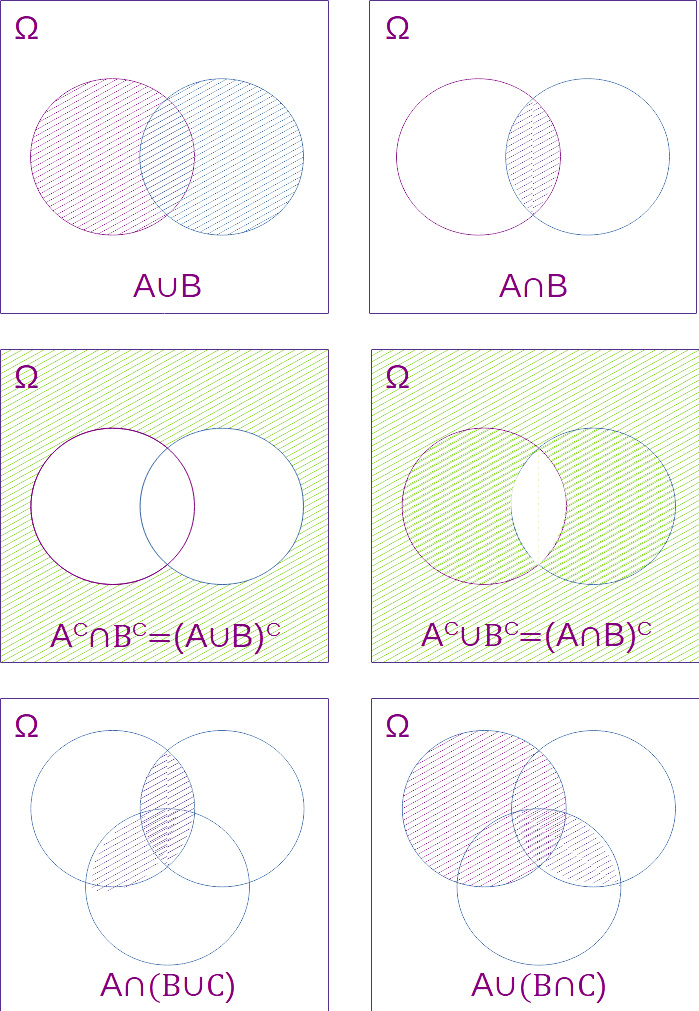
\includegraphics[width=5.30208in,height=\textheight]{Vennd.png}

}

\caption{\label{fig-venn}Diagramas de Venn}

\end{figure}

Algunas de las leyes mencionadas anteriormente se ilustran en los
diagramas de Venn en la Figura~\ref{fig-venn}. Aunque se utilizará
libremente cualquiera de las leyes mencionadas, podría resultar
instructivo proporcionar una prueba de una de ellas para ilustrar la
técnica. Se considera el siguiente ejemplo:

\begin{tcolorbox}[enhanced jigsaw, toprule=.15mm, left=2mm, opacitybacktitle=0.6, titlerule=0mm, bottomrule=.15mm, arc=.35mm, coltitle=black, colframe=quarto-callout-caution-color-frame, colbacktitle=quarto-callout-caution-color!10!white, bottomtitle=1mm, opacityback=0, toptitle=1mm, title={Ejemplo}, rightrule=.15mm, breakable, colback=white, leftrule=.75mm]

Demostrar que \((A \cup B)^c = A^c \cap B^c\).

\begin{proof}

Según la definición, dos conjuntos son iguales si cada uno está
contenido en el otro. Primero se demuestra que
\((A\cup B)^c \subset A^c\cap B^c\) al probar que si
\(\omega \in (A\cup B)^c\), entonces \(\omega \in A^c \cap B^c\). Ahora
bien, \(\omega \in (A\cup B)^c\) implica que \(\omega \notin A \cup B\),
lo cual implica que \(\omega \notin A\) y \(\omega \notin B\), lo que a
su vez implica que \(\omega \in A^c\) y \(\omega \in B^c\); es decir,
\(\omega \in A^c\cap B^c\). A continuación se demuestra que
\(A^c \cap B^c \subset (A\cup B)^c\). Sea \(\omega \in A^c \cap B^c\),
lo que significa que \(\omega\) pertenece tanto a \(A^c\) como a
\(B^c\). Entonces, \(\omega \notin A \cup B\), ya que de lo contrario
\(\omega\) debería pertenecer al menos a uno de los conjuntos \(A\) o
\(B\), lo cual contradice que \(\omega\) pertenezca tanto a \(A^c\) como
a \(B^c\); sin embargo, \(\omega \notin A \cup B\) implica que
\(\omega \in (A\cup B)^c\), lo que completa la prueba.

\end{proof}

\end{tcolorbox}

Se han definido la unión y la intersección de dos conjuntos; estas
definiciones se extienden inmediatamente a más de dos conjuntos, de
hecho, a un número arbitrario de conjuntos. Es costumbre distinguir
entre los conjuntos en una colección de subconjuntos de \(\Omega\)
asignándoles nombres en forma de subíndices.

Se considera el conjunto de índices \(\Lambda\) como el catálogo de
nombres o índices. A \(\Lambda\) también se le denomina conjunto de
índices. Por ejemplo, si se tiene interés únicamente en dos conjuntos,
entonces el conjunto de índices \(\Lambda\) incluye solo dos índices,
por ejemplo, 1 y 2; así, \(\Lambda=\{1,2\}\).

\begin{definition}[Unión e intersección de
conjuntos]\protect\hypertarget{def-UI}{}\label{def-UI}

Sea \(\Lambda\) un conjunto de índices y
\(\{A_\lambda: \lambda \in \Lambda\}= \{A_\lambda\}\), una colección de
subconjuntos de \(\Omega\) indexados por \(\Lambda\). El conjunto de
puntos que consiste en todos los puntos que pertenecen a \(A_\lambda\)
para al menos un \(\lambda\) se denomina unión de los conjuntos
\(\{A_\lambda\}\) y se denota como
\(\bigcup\limits_{\lambda\in \Lambda} A_\lambda\). El conjunto de puntos
que consiste en todos los puntos que pertenecen a \(A_\lambda\) para
cada \(\lambda\) se denomina intersección de los conjuntos
\(\{A_\lambda\}\) y se denota como
\(\bigcap\limits_{\lambda\in\Lambda} A_\lambda\). Si \(\Lambda\) está
vacío, entonces se define
\(\bigcup\limits_{\lambda\in \Lambda} A_\lambda = \emptyset\) y
\(\bigcap\limits_{\lambda\in\Lambda} A_\lambda=\Omega\).

\end{definition}

Uno de los teoremas más fundamentales que relaciona las uniones,
intersecciones y complementos para una colección arbitraria de conjuntos
se debe a De Morgan.

\begin{theorem}[Teorema de De
Morgan]\protect\hypertarget{thm-morgan}{}\label{thm-morgan}

Sea \(\Lambda\) un conjunto de índices y \(\{A_\lambda\}\) una colección
de subconjuntos de \(\Omega\) indexados por \(\Lambda\). Entonces,

\begin{enumerate}
\def\labelenumi{\roman{enumi}.}
\item
  \(\left(\bigcup\limits_{\lambda\in\Lambda} A_\lambda\right)^c = \bigcap\limits_{\lambda\in\Lambda} A_\lambda^c\)
\item
  \(\left(\bigcap\limits_{\lambda\in\Lambda} A_\lambda\right)^c = \bigcup\limits_{\lambda\in\Lambda} A_\lambda^c\)
\end{enumerate}

\end{theorem}

\begin{definition}[Disjuntos o mutuamente
excluyentes]\protect\hypertarget{def-disjunto}{}\label{def-disjunto}

Los subconjuntos \(A\) y \(B\) de \(\Omega\) se definen como mutuamente
excluyentes o disjuntos si \(A\cap B=\emptyset\). Los subconjuntos
\(A_1, A_2, \ldots\) se definen como mutuamente excluyentes si
\(A_i\cap A_j=\emptyset\) para cada \(i\neq j\).

\end{definition}

\hypertarget{probabilidad}{%
\section{Probabilidad}\label{probabilidad}}

Una de las herramientas fundamentales de la estadística es la
probabilidad, la cual tuvo sus inicios formales con los juegos de azar
en el siglo XVII. Los juegos de azar, como su nombre indica, involucran
acciones como girar una rueda de ruleta, lanzar dados, lanzar una
moneda, sacar una carta, entre otros, en los que el resultado de un
evento es incierto. No obstante, se reconoce que aunque el resultado de
cada evento en particular pueda ser incierto, existe un patrón
predecible a largo plazo. Por ejemplo, se sabe que en múltiples
lanzamientos de una moneda ideal (equilibrada y simétrica),
aproximadamente la mitad de los resultados serán caras. Es esta
regularidad predecible a largo plazo la que permite a las casas de juego
mantener sus negocios.

Un tipo similar de incertidumbre y regularidad a largo plazo se observa
con frecuencia en la ciencia experimental. Por ejemplo, en la ciencia de
la genética no se puede determinar con certeza si una descendencia será
masculina o femenina, pero a largo plazo se sabe aproximadamente qué
porcentaje de descendencia será de cada sexo. De manera similar, una
compañía de seguros de vida no puede predecir qué personas en los
Estados Unidos morirán a los 50 años, pero puede hacer predicciones
precisas sobre cuántas personas morirán a esa edad en promedio.

Para brindar una idea de lo que es la probabilidad, Mood, Graybill, y
Boes (1986) proporciona las siguientes definiciones:

\begin{definition}[Probabilidad
clásica]\protect\hypertarget{def-pclas}{}\label{def-pclas}

Si un experimento aleatorio puede resultar en \(n\) resultados
mutuamente excluyentes e igualmente probables y si \(s\) de estos
resultados tienen un atributo \(A\), entonces la probabilidad de \(A\)
es la fracción \(s/n\).

\end{definition}

\begin{definition}[Probabilidad
frecuentista]\protect\hypertarget{def-pfrec}{}\label{def-pfrec}

Suponiendo que después de \(n\) repeticiones, para valores muy grandes
de \(n\), un evento \(A\) puede ocurrir \(s\) veces. Entonces \(p=s/n\).

\end{definition}

Estas definiciones, a pesar de su intuición, presentan limitaciones
significativas. Por ejemplo, la primera definición es circular, ya que
la frase ``igualmente probables'' es justamente lo que se intenta
definir. Además, la segunda definición no especifica los valores de
\(n\), lo cual puede generar ambigüedad. Estas definiciones son
consideradas antiguas, pero aún pueden brindar una comprensión general
del concepto de \textbf{probabilidad}.

\hypertarget{espacio-muestral-y-eventos}{%
\subsection{Espacio muestral y
eventos}\label{espacio-muestral-y-eventos}}

A continuación, se presentarán algunas definiciones que resultarán de
gran utilidad para adquirir un mayor conocimiento sobre el concepto de
probabilidad.

\begin{definition}[Espacio
muestral]\protect\hypertarget{def-espm}{}\label{def-espm}

El espacio muestral, denotado por \(\Omega\), es la colección o
totalidad de todos los posibles resultados de un experimento conceptual.

\end{definition}

Un resultado particular, es decir, un elemento del espacio muestral
\(\Omega\), se denomina un \textbf{\emph{punto muestral}} o una
\textbf{\emph{muestra}}.

\begin{definition}[Evento]\protect\hypertarget{def-evento}{}\label{def-evento}

Un evento \(A\) es un subconjunto del espacio muestral \(\Omega\), es
decir, es un conjunto de resultados.

\end{definition}

\begin{definition}[Espacio de
eventos]\protect\hypertarget{def-espev}{}\label{def-espev}

La clase de todos los eventos asociados a un experimento dado se define
como el espacio de eventos y se denotará por \(\mathfrak{F}\).

\end{definition}

\begin{definition}[Evento
particular]\protect\hypertarget{def-evpart}{}\label{def-evpart}

El evento \(\{\omega\}\), que está constituido por un solo punto
\(\omega \in \Omega\), se denomina \emph{evento muestral} o \emph{punto
muestral}.

\end{definition}

Las definiciones anteriores no definen con precisión lo que es un
evento. Un evento siempre será un subconjunto del espacio muestral, pero
para espacios muestrales suficientemente grandes, no todos los
subconjuntos serán eventos. Por lo tanto, la clase de todos los
subconjuntos del espacio muestral no necesariamente corresponderá al
espacio de eventos. Sin embargo, se observará que la clase de todos los
eventos siempre se puede seleccionar lo suficientemente grande como para
incluir todos aquellos subconjuntos (eventos) cuya probabilidad se desee
analizar. Si el espacio muestral consta solo de un número finito de
puntos, entonces el espacio de eventos correspondiente será la clase de
todos los subconjuntos del espacio muestral.

Los conceptos presentados se ilustran con unos ejemplos muy simples;

\begin{tcolorbox}[enhanced jigsaw, toprule=.15mm, left=2mm, opacitybacktitle=0.6, titlerule=0mm, bottomrule=.15mm, arc=.35mm, coltitle=black, colframe=quarto-callout-caution-color-frame, colbacktitle=quarto-callout-caution-color!10!white, bottomtitle=1mm, opacityback=0, toptitle=1mm, title={Ejemplo (\textbf{\emph{Lanzamiento de una moneda}})}, rightrule=.15mm, breakable, colback=white, leftrule=.75mm]

Considerando el experimento de lanzar una moneda, este experimento es
uno de los más sencillos, pero permite representar claramente los
conceptos. El espacio muestral estaría conformado por
\(\Omega = \{A, S\}\), donde \(A\) representa el resultado de que caiga
águila y \(S\) representa el resultado de que caiga sol. El conjunto
\(\mathfrak{F}\) podría estar representado por \(\{\{A\}, \{S\}\}\), que
también es un subconjunto de \(\Omega\).

Es importante destacar que el conjunto vacío \(\emptyset\) y el conjunto
completo \(\Omega\) también son subconjuntos de \(\Omega\), pero
generalmente no se consideran eventos de interés en este contexto.

\end{tcolorbox}

\begin{tcolorbox}[enhanced jigsaw, toprule=.15mm, left=2mm, opacitybacktitle=0.6, titlerule=0mm, bottomrule=.15mm, arc=.35mm, coltitle=black, colframe=quarto-callout-caution-color-frame, colbacktitle=quarto-callout-caution-color!10!white, bottomtitle=1mm, opacityback=0, toptitle=1mm, title={Ejemplo (\textbf{\emph{Lanzamiento de un dado}})}, rightrule=.15mm, breakable, colback=white, leftrule=.75mm]

Considerando el experimento de lanzar un dado de \(6\) caras. El espacio
muestral \(\Omega\) se define como

\[ \Omega = \{1,2,3,4,5,6\}. \]

Un punto muestral podría ser un resultado específico, por ejemplo,
\(\{1\}\). Todos los subconjuntos posibles de resultados constituirían
el conjunto \(\mathfrak{F}\). Se definen los eventos \(A\), que
representa el evento de obtener un resultado par; \(B\), que representa
el evento de obtener un resultado impar; y \(C\), que representa el
evento de obtener un resultado mayor a 3. Por lo tanto, se tiene:

\[ A= \{2,4,6\},\quad B=\{1,3,5\},\quad C=\{4,5,6\}. \]

Se observa que el evento de la unión de los eventos \(B\) y \(C\),
denotado como \(B\cup C\), es igual a \(\{1, 3, 4, 5, 6\}\), el cual
también es un evento en el espacio muestral \(\Omega\). Finalmente, se
destaca que los eventos \(A\) y \(B\) no tienen elementos en común, es
decir, \(A \cap B = \emptyset\). Por lo tanto, se dice que estos eventos
son ajenos, mutuamente excluyentes o disjuntos.

\end{tcolorbox}

La definición de espacio muestral es precisa y satisfactoria, mientras
que las definiciones de evento y espacio de eventos no son completamente
satisfactorias. Se mencionó que si el espacio muestral era
``suficientemente grande'', no todos los subconjuntos del espacio
muestral serían eventos; sin embargo, no se especificó exactamente qué
subconjuntos serían eventos y cuáles no lo serían. En lugar de
desarrollar las matemáticas necesarias para definir con precisión qué
subconjuntos de \(\Omega\) constituyen nuestro espacio de eventos
\(\mathfrak{F}\), se pueden enunciar algunas propiedades de
\(\mathfrak{F}\) que parecen razonables requerir.

\begin{enumerate}
\def\labelenumi{\roman{enumi}.}
\item
  \(\Omega \in \mathfrak{F}\).
\item
  Si \(A\in\mathfrak{F}\), entonces \(A^c\in \mathfrak{F}\).
\item
  Si \(A_1\) y \(A_2\in \mathfrak{F}\), entonces
  \(A_1\cup A_2\in \mathfrak{F}\).
\end{enumerate}

Se mencionó anteriormente que el interés principal radica en los eventos
debido a la probabilidad de que ocurran. Por lo tanto, es deseable que
\(\mathfrak{F}\) incluya \(\Omega\), el evento seguro. Además, si \(A\)
es un evento, lo que significa que se puede hablar sobre la probabilidad
de que ocurra \(A\), entonces \(A^c\) también debería ser un evento para
poder hablar sobre la probabilidad de que \(A\) no ocurra. De manera
similar, si \(A_1\) y \(A_2\) son eventos, entonces \(A_1\cup A_2\)
también debería ser un evento.

Cualquier colección de eventos con propiedades (i.) y (iii.) se denomina
álgebra booleana, o simplemente álgebra, de eventos. Cabe señalar que la
colección de todos los subconjuntos de \(\Omega\) satisface
necesariamente las propiedades mencionadas anteriormente. Varios
resultados se derivan de las propiedades asumidas anteriormente de
\(\mathfrak{F}\).

\hypertarget{definiciuxf3n-de-probabilidad}{%
\subsection{Definición de
probabilidad}\label{definiciuxf3n-de-probabilidad}}

En esta sección se presenta la definición axiomática de probabilidad.
Aunque esta definición formal de probabilidad por sí sola no permite
asignar probabilidades reales a eventos que consisten en ciertos
resultados de experimentos aleatorios, es otra de una serie de
definiciones que conducen a ese objetivo. Dado que la probabilidad, al
igual que los conceptos que se presentarán, se define como una función
particular, se inicia esta subsección con una revisión del concepto de
función

\begin{definition}[Función]\protect\hypertarget{def-funcion}{}\label{def-funcion}

Una función, llamada \(f(\cdot)\), con dominio \(A\) y contradominio
\(B\), es una colección de pares ordenados, llamados \((a,b)\), que
cumplen las siguientes condiciones:

\begin{enumerate}
\def\labelenumi{\roman{enumi}.}
\item
  \(a\in A\) y \(b\in B\)
\item
  Cada \(a\in A\) aparece como el primer elemento de algún par ordenado
  en la colección (cada \(b\in B\) no necesariamente es el segundo
  elemento de algún par ordenado)
\item
  Ningún par ordenado en la colección tiene el mismo primer elemento que
  otro par ordenado distinto.
\end{enumerate}

\end{definition}

Si \((a,b)\in f(\cdot)\), se escribe \(b=f(a)\) (se lee ``\(b\) es igual
a \(f\) de \(a\)'') y se denomina \(f(a)\) como el valor de \(f(\cdot)\)
en \(a\). Para cualquier \(a\in A\), \(f(a)\) es un elemento de \(B\);
mientras que \(f(\cdot)\) es un conjunto de pares ordenados. El conjunto
de todos los valores de \(f(\cdot)\) se denomina rango de \(f(\cdot)\);
es decir, el rango de
\(f(\cdot)=\{b\in B:b=f(a) \text{ para algún } a\in A\}\) y siempre es
un subconjunto del contradominio \(B\), pero no necesariamente igual a
él. \(f(a)\) también se denomina imagen de \(a\) bajo \(f(\cdot)\), y
\(a\) se denomina preimagen de \(f(a)\).

\begin{tcolorbox}[enhanced jigsaw, toprule=.15mm, left=2mm, opacitybacktitle=0.6, titlerule=0mm, bottomrule=.15mm, arc=.35mm, coltitle=black, colframe=quarto-callout-caution-color-frame, colbacktitle=quarto-callout-caution-color!10!white, bottomtitle=1mm, opacityback=0, toptitle=1mm, title={Ejemplo}, rightrule=.15mm, breakable, colback=white, leftrule=.75mm]

Sean \(f_1(\cdot)\) y \(f_2(\cdot)\) dos funciones con la recta real
como su dominio y contradominio, definidas por

\[ f_1(\cdot)=\{(x,y): y=x^3+1, -\infty< x< \infty\} \]

y

\[ f_2(\cdot)=\{(x,y): y=x^2, -\infty<x< \infty\} \]

El rango de \(f_1(\cdot)\) es el contradominio, que es toda la recta
real, pero el rango de \(f_2(\cdot)\) son todos los números reales no
negativos, que no es igual al contradominio.

\end{tcolorbox}

De particular interés será una clase de funciones conocidas como
funciones indicadoras.

\begin{definition}[Función
indicadora]\protect\hypertarget{def-f_ind}{}\label{def-f_ind}

Sea \(\Omega\) cualquier espacio con puntos \(\omega\) y \(A\) cualquier
subconjunto de \(\Omega\). La función indicadora de \(A\), denominada
\(I_A(\cdot)\), es la función con dominio \(\Omega\) y contradominio
formado por dos números reales, 0 y 1, definida por

\[ I_A(\omega)= \left\{\begin{array}{lcc} 1 & si & \omega \in A\\ \\0 & si & \omega \notin A \end{array}\right. \]

\(I_A(\cdot)\) claramente ``indica'' el conjunto \(A\).

\end{definition}

\textbf{\emph{Propiedades de la función indicadora.}}

Sea \(\Omega\) cualquier espacio y \(\mathfrak{F}\) cualquier colección
de subconjuntos de \(\Omega\):

\begin{enumerate}
\def\labelenumi{\roman{enumi}.}
\item
  \(I_A(\omega)= 1- I_{A^c}(\omega)\) para cada \(A\in \mathfrak{F}\).
\item
  \(I_{A_1A_2\cdots A_n}(\omega)= I_{A_1}(\omega)\cdot I_{A_2}(\omega)\cdots I_{A_n}(\omega)\)
  para \(A_1,\ldots, A_n\in \mathfrak{F}\).
\item
  \(I_{A_1\cup A_2\cup\cdots\cup A_n}(\omega)= \max{[I_{A_1}(\omega), I_{A_2}(\omega),\ldots, I_{A_n}(\omega)]}\)
  para \(A_1, \ldots, A_n \in\mathfrak{F}\).
\item
  \(I_A^2(\omega)= I_A(\omega)\) para cada \(A\in\mathfrak{F}\).
\end{enumerate}

La función indicadora será utilizada para ``indicar'' subconjuntos de la
recta real; por ejemplo;

\[I_{\{[0,1)\}}(x)= I_{[0,1)}(x)=\left\{ \begin{array}{lcc} 1 & \text{si} & 0\leq x<1\\ \\ 0 & \text{ otro caso} \end{array} \right. \]

y si \(I^+\) denota el conjunto de números enteros positivos,

\[ I_{I^+}(X)=\left\{\begin{array}{lcc} 1 & \text{si $x$ es algún entero positivo}\\ \\ 0 & \text{otro caso}\end{array}\right. \]

Otro tipo de función del cual se tendrá ocasión de discutir es la
función de conjunto definida como cualquier función que tiene como
dominio una colección de conjuntos y como contradominio la recta real,
incluyendo posiblemente el infinito. A continuación se muestra un
ejemplos de función de conjunto.

\begin{tcolorbox}[enhanced jigsaw, toprule=.15mm, left=2mm, opacitybacktitle=0.6, titlerule=0mm, bottomrule=.15mm, arc=.35mm, coltitle=black, colframe=quarto-callout-caution-color-frame, colbacktitle=quarto-callout-caution-color!10!white, bottomtitle=1mm, opacityback=0, toptitle=1mm, title={Ejemplo}, rightrule=.15mm, breakable, colback=white, leftrule=.75mm]

Sea \(\Omega\) el espacio muestral correspondiente al experimento de
lanzar dos dados, y sea \(\mathfrak{F}\) la colección de todos los
subconjuntos de \(\Omega\). Para cualquier \(A\in\mathfrak{F}\), se
define \(N(A)\) como el número de resultados, o puntos en \(\Omega\),
que están en \(A\). Entonces, \(N(\emptyset)=0\), \(N(\Omega)=36\) y
\(N(A)=6\) si \(A\) es el evento que contiene aquellos resultados que
tienen un total de siete puntos arriba.

\end{tcolorbox}

La función de tamaño del conjunto aludida en el ejemplo anterior puede
ser definida, en general, para cualquier conjunto \(A\) como el número
de puntos en \(A\), donde \(A\) es un miembro de una colección
arbitraria de conjuntos \(\mathfrak{F}\).

La función de probabilidad que se definirá será una función de conjunto
particular.

\begin{definition}[Función de
probabilidad]\protect\hypertarget{def-fprob}{}\label{def-fprob}

Sea \(A\) un evento del espacio muestral \(\Omega\). Una función
\(P: \mathfrak{F} \to [0,1]\) es llamada función de probabilidad y
\(P(A)\) se denomina la \emph{probabilidad} del evento \(A\) si se
cumplen los siguientes axiomas:

\begin{enumerate}
\def\labelenumi{\roman{enumi}.}
\item
  \textbf{\emph{No negatividad}}: Para todo evento \(A\) en
  \(\mathfrak{F}\), la probabilidad \(P(A)\) es un número no negativo,
  es decir, \(P(A) \geq 0\).
\item
  \textbf{\emph{Probabilidad unitaria}}: La probabilidad del espacio
  muestral completo \(\Omega\) es igual a 1, es decir,
  \(P(\Omega) = 1\).
\item
  \textbf{\emph{Aditividad}}: Para cualquier colección de eventos
  mutuamente excluyentes \(A_1, A_2, A_3, \ldots\), la probabilidad de
  la unión de estos eventos es igual a la suma de las probabilidades
  individuales, es decir,
  \[P\left(\bigcup_{i=1}^\infty A_i\right) = \sum_{i=1}^\infty P(A_i)\]
\end{enumerate}

\end{definition}

Estos axiomas establecen las propiedades esenciales que debe cumplir una
función de probabilidad para ser considerada válida. Cumplir con estos
axiomas garantiza que la función de probabilidad asigna valores
coherentes y consistentes a los eventos en el espacio muestral.

A partir de los axiomas, se derivan otras propiedades que nos ayudarán a
posible calcular las probabilidades de varios eventos.

\begin{enumerate}
\def\labelenumi{\roman{enumi}.}
\item
  \(P(\emptyset)=0\).
\item
  Si \(A_1, \ldots, A_n\) son eventos mutuamente excluyentes en
  \(\mathfrak{F}\), entonces
  \[P\left(\bigcup\limits_{i=1}^n A_i\right)= \sum\limits_{i=1}^n P(A_i).\]
\item
  Si \(A\) es un evento en \(\mathfrak{F}\), entonces
  \[P(A^c)= 1-P(A).\]
\item
  Si \(A,B\in\mathfrak{F}\), entonces

  \[P(A)= P(A\cap B)+ P(A\cap B^c)\]

  y \[P(A-B)=P(A\cap B^c)= P(A)-P(A\cap B).\]
\item
  Si \(A,B\in \mathfrak{F}\) y \(A\subset B\), entonces
  \(P(A)\leq P(B)\).
\item
  Para cualesquiera dos eventos \(A,B\in \mathfrak{F}\);
  \[P(A\cup B)= P(A)+P(B)-P(A\cap B).\]Más generalmente, para eventos
  \(A_1, A_2, \ldots, A_n\in \mathfrak{F}\)
\end{enumerate}

\[ P\left(\bigcup\limits_{i=1}^n A_i\right) = \sum_{j=1}^nP(A_j)-{\sum\sum}_{i<j} P(A_i\cap A_j)+\sum\sum\sum_{i<j<k}P(A_i\cap A_j\cap A_k)\\ -\cdots+(-1)^{n+1}P(A_1\cap \ldots\cap A_n) \]

\begin{theorem}[Desigualdad de
Boole]\protect\hypertarget{thm-boole}{}\label{thm-boole}

Si \(A_1, A_2, \ldots, A_n\in\mathfrak{F}\), entonces

\[P\left(\bigcup_{i=1}^n A_i\right)\leq \sum_{i=1}^n P(A_i)\]

\end{theorem}

Finalmente se concluye esta subsección con la siguiente definición;

\begin{definition}[Espacio de
probabilidad]\protect\hypertarget{def-Ep}{}\label{def-Ep}

Un espacio de probabilidad es la terna \((\Omega, \mathfrak{F}, P)\),
donde \(\Omega\) es un espacio muestral, \(\mathfrak{F}\) es una
colección (asumida como un álgebra) de eventos (cada uno un subconjunto
de \(\Omega\)), y \(P\) es una función de probabilidad con dominio
\(\mathfrak{F}\).

\end{definition}

\hypertarget{probabilidad-condicional}{%
\subsection{Probabilidad condicional}\label{probabilidad-condicional}}

En ocasiones, es de interés conocer la probabilidad de un evento, dado
que haya ocurrido otro. En este sentido, se define la probabilidad
condicional.

\begin{definition}[Probabilidad
condicional]\protect\hypertarget{def-pcond}{}\label{def-pcond}

Sean \(A\) y \(B\) dos eventos en \(\mathfrak{F}\) del espacio de
probabilidad dado \((\Omega, \mathfrak{F}, P)\). La probabilidad
condicional del evento \(A\) dado el evento \(B\), denotada por
\(P(A|B)\), se define como sigue;

\[P(A|B)= \frac{P(A\cap B)}{P(B)}\qquad\text{si }\quad P(B)>0,\]

y se deja sin definir si \(P(B)=0\).

\end{definition}

\begin{remark}

Una fórmula que es evidente a partir de la definición es
\[P(A\cap B)= P(A|B)P(B)=P(B|A)P(A)\] si tanto \(P(A)\) como \(P(B)\)
son diferentes de cero. Esta fórmula relaciona \(P(A|B)\) con \(P(B|A)\)
en términos de las probabilidades incondicionales \(P(A)\) y \(P(B)\).

\end{remark}

De la definición anterior, se desprenden las siguientes propiedades de
la función de probabilidad condicional. Se asume que el espacio de
probabilidad \((\Omega, \mathfrak{F}, P)\) está dado, y se considera que
\(B\in\mathfrak{F}\) cumple con \(P[B]>0\).

\begin{enumerate}
\def\labelenumi{\roman{enumi}.}
\item
  \(P(\emptyset| B)=0\).
\item
  Si \(A_1, A_2, \ldots, A_n\) son eventos mutuamente excluyentes en
  \(\mathfrak{F}\), entonces

  \[P\left(\bigcup_{i=1}^n A_i|B\right)= \sum_{i=1}^n P(A_i|B).\]
\item
  Si \(A\) es un evento en \(\mathfrak{F}\), entonces
  \(P(A^c| B)=1-P(A|B)\).
\item
  Si \(A_1, A_2\in \mathfrak{F}\), entonces
  \(P(A_1|B)=P(A_1\cap A_2|B)+ P(A_1\cap A_2^c|B)\).
\item
  Para cualesquiera dos eventos \(A_1,A_2\in \mathfrak{F}\)

  \[P(A_1\cup A_2|B)=P(A_1|B)+P(A_2|B)-P(A_1\cap A_2|B).\]
\item
  Si \(A_1, A_2\in\mathfrak{F}\) y \(A_1\subset A_2\), entonces
  \(P(A_1|B)\leq P(A_2|B)\).
\item
  Si \(A_1, A_2,\ldots, A_n\in\mathfrak{F}\), entonces

  \[P\left(\bigcup_{i=1}^n A_i|B\right)\leq \sum_{i=1}^n P(A_i|B).\]
\end{enumerate}

A continuación se mencionan unos teoremas de gran importancia. La
aplicación de dichos teoremas se ilustran con unos ejemplos.

\begin{theorem}[Teorema de probabilidades
totales]\protect\hypertarget{thm-ptotales}{}\label{thm-ptotales}

Para un espacio de probabilidad dado \((\Omega, \mathfrak{F}, P)\), si
\(B_1, B_2, \ldots, B_n\) es una colección de eventos mutuamente
disjuntos en \(\mathfrak{F}\) que satisfacen
\(\Omega = \bigcup\limits_{j=1}^n B_j\) y \(P(B_j)>0\) para
\(j=1,\ldots, n\), entonces para cada \(A\in \mathfrak{F}\),
\[P(A)=\sum_{j=1}^n P(A|B_j)P(B_j).\]

\begin{proof}

Se observa que \(A=\bigcup\limits_{j=1}^n A\cap B_j\) y los conjuntos
\(A\cap B_j\) son mutuamente disjuntos; por lo tanto,

\[P(A)=P\left(\bigcup_{j=1}^n A\cap B_j\right)=\sum_{j=1}^n P(A\cap B_j)= \sum_{j=1}^n P(A|B_j)P(B_j)\]

\end{proof}

\end{theorem}

\begin{tcolorbox}[enhanced jigsaw, toprule=.15mm, left=2mm, opacitybacktitle=0.6, titlerule=0mm, bottomrule=.15mm, arc=.35mm, coltitle=black, colframe=quarto-callout-caution-color-frame, colbacktitle=quarto-callout-caution-color!10!white, bottomtitle=1mm, opacityback=0, toptitle=1mm, title={Ejemplo (\textbf{\emph{Seleccionar una pelota de varias urnas}})}, rightrule=.15mm, breakable, colback=white, leftrule=.75mm]

Hay dos urnas con pelotas de diferentes colores, todas del mismo tamaño.
En la primera urna, hay tres pelotas rojas, tres blancas y cuatro
negras; en la segunda urna, hay cuatro pelotas rojas, tres blancas y una
negra. Se elige una urna al azar y se saca una pelota de ella. ¿Cuál es
la probabilidad de que la pelota extraída sea blanca?

\begin{solution}

Se debe observar que la elección de las urnas constituye dos eventos
mutuamente excluyentes, ya que la unión de ambos eventos constituye el
espacio muestral (todas las pelotas están en la primera o segunda urna).
Se denomina \(B_1\) al evento de seleccionar la primera urna, y \(B_2\)
al evento de seleccionar la segunda urna.

El evento de extraer una pelota blanca puede tener lugar tanto al elegir
la primera urna como al elegir la segunda urna, lo que permite la
aplicación de la fórmula del teorema de probabilidades totales. Se
designa como \(A\) al evento de seleccionar una pelota blanca.

De esta manera,

\[
P(A)= \sum_{j=1}^2 P(A|B_j)P(B_j)=P(A|B_1)P(B_1)+P(A|B_2)P(B_2)
\]

Bajo la premisa de probabilidades equivalentes, se tiene que
\(P(B_1)=P(B_2)=\frac{1}{2}\), \(P(A|B_1)=\frac{3}{10}\) y
\(P(A|B_2)=\frac{3}{8}\), por lo que la probabilidad de elegir una
pelota blanca es \(0.3375\).

\end{solution}

\end{tcolorbox}

\begin{theorem}[Teorema de
Bayes]\protect\hypertarget{thm-bayes}{}\label{thm-bayes}

Para un espacio de probabilidad dado \((\Omega, \mathfrak{F}, P)\), si
\(B_1, B_2, \ldots, B_n\) es una colección de eventos mutuamente
disjuntos en \(\mathfrak{F}\) que satisfacen
\(\Omega=\bigcup\limits_{j=1}^n B_j\) y \(P(B_j)>0\) para
\(j=1,\ldots, n\), entonces para cada \(A\in\mathfrak{F}\) para el cual
\(P(A)>0\)

\[P(B_k|A)= \frac{P(A|B_k)P(B_k)}{\sum\limits_{j=1}^n P(A|B_j)P(B_j)}.\]

\begin{proof}

Se observa que

\[P(B_k|A)= \frac{P(B_k\cap A)}{P(A)}=\frac{P(A|B_k)P(B_k)}{\sum\limits_{j=1}^n P(A|B_j)P(B_j)}\]

utilizando tanto la definición de probabilidad condicional como el
teorema de probabilidad total.

\end{proof}

\end{theorem}

\begin{tcolorbox}[enhanced jigsaw, toprule=.15mm, left=2mm, opacitybacktitle=0.6, titlerule=0mm, bottomrule=.15mm, arc=.35mm, coltitle=black, colframe=quarto-callout-caution-color-frame, colbacktitle=quarto-callout-caution-color!10!white, bottomtitle=1mm, opacityback=0, toptitle=1mm, title={Ejemplo (\textbf{\emph{Seleccionar una pelota de varias urnas}})}, rightrule=.15mm, breakable, colback=white, leftrule=.75mm]

Considérese el problema de las urnas. Teniendo en cuenta que la pelota
extraída fue blanca, ¿cuál es la probabilidad de que haya provenido de
la primera urna?

\begin{solution}

Debe calcularse la probabilidad \(P(B_1|A)\). Al utilizar el teorema de
Bayes, solo se realiza la sustitución en la fórmula y se obtiene que la
probabilidad resultante es \(0.4444\).

\end{solution}

\end{tcolorbox}

\begin{theorem}[Regla de
multiplicación]\protect\hypertarget{thm-mult}{}\label{thm-mult}

Para un espacio de probabilidad dado \((\Omega, \mathfrak{F}, P)\), sean
\(A_1, A_2, \ldots, A_n\) eventos pertenecientes a \(\mathfrak{F}\) para
los cuales \(P(A_1\cdots A_{n-1})>0\); entonces

\[P(A_1A_2\cdots A_n)= P(A_1)P(A_2|A_1)P(A_3|A_1A_2)\cdots P(A_n|A_1\cdots A_{n-1})\]

\end{theorem}

\hypertarget{independencia-de-eventos}{%
\subsection{Independencia de eventos}\label{independencia-de-eventos}}

Si \(P(A|B)\) no depende del evento \(B\), es decir, \(P(A|B)=P(A)\),
entonces parecería natural decir que el evento \(A\) es independiente
del evento \(B\). Esto se establece en la siguiente definición.

\begin{definition}[Eventos
independientes]\protect\hypertarget{def-evind}{}\label{def-evind}

Para un espacio de probabilidad dado \((\Omega, \mathfrak{F}, P)\), sean
\(A\) y \(B\) dos eventos en \(\mathfrak{F}\). Los eventos \(A\) y \(B\)
se definen como \emph{independientes} si y solo si se cumple alguna de
las siguientes condiciones:

\begin{enumerate}
\def\labelenumi{\roman{enumi}.}
\item
  \(P(A\cap B)= P(A)P(B)\).
\item
  \(P(A|B)=P(A)\) si \(P(B)>0\).
\item
  \(P(B|A)=P(B)\) si \(P(A)>0\).
\end{enumerate}

\end{definition}

De la definición anterior, se desprende lo siguiente

\leavevmode\vadjust pre{\hypertarget{thm}{}}%
Si \(A\) y \(B\) son dos eventos independientes definidos en un espacio
de probabilidad dado \((\Omega, \mathfrak{F}, P)\), entonces los
siguientes eventos también son independientes

\begin{enumerate}
\def\labelenumi{\roman{enumi}.}
\item
  \(A\) y \(B^c\),
\item
  \(A^c\) y \(B\),
\item
  \(A^c\) y \(B^c\).
\end{enumerate}

\begin{remark}

No debe confundirse los términos \textbf{eventos independientes} y
\textbf{eventos disjuntos}. De hecho, los eventos disjuntos suelen ser
muy dependientes por que la ocurrencia de uno implica la no ocurrencia
del otro. El único evento que es independiente y ajeno es el vacío
\(\emptyset\).

\end{remark}

La noción de eventos independientes puede ser extendido a más de dos
eventos como se sigue;

\begin{definition}[Independencia de varios
eventos]\protect\hypertarget{def-ive}{}\label{def-ive}

Para un espacio de probabilidad dado \((\Omega, \mathfrak{F}, P)\), sean
\(A_1, A_2, \ldots, A_n\) eventos en \(\mathfrak{F}\). Los eventos
\(A_1, A_2, \ldots, A_n\) se definen como independientes si y solo si
\(P\left(\bigcap\limits_{i=1}^n A_i\right)=\prod\limits_{i=1}^n P(A_i)\)

\end{definition}

\hypertarget{variables-aleatorias}{%
\subsection{Variables aleatorias}\label{variables-aleatorias}}

Hasta el momento se conoce cómo asignar probabilidades a eventos del
espacio muestral, sin embargo en la práctica esto no siempre es posible
ya que sería complicado mencionar o enumerar todos los elementos del
espacio muestral.

Por esta razón es necesario ``traducir'' dichos eventos a números
reales. Esto es posible mediante el uso de \emph{variables aleatorias}.

\begin{definition}[Variable
aleatoria]\protect\hypertarget{def-va}{}\label{def-va}

Para un espacio de probabilidad dado \((\Omega, \mathfrak{F}, P)\), una
variable aleatoria, denotada por \(X\) o \(X(\cdot)\), es una función
con dominio \(\Omega\) y contradominio la recta real. La función
\(X(\cdot)\) debe ser tal si \(\omega\in\Omega\) entonces
\(X(\omega)\in\mathbb R\). Si \(B\subset \mathbb R\) entonces
\(X^{-1}(B)\in\mathfrak{F}\), donde
\[X^{-1}(B)=\{\omega\in\Omega| X(\omega\in B)\}.\]

\end{definition}

Existen dos tipos de variables aleatorias: discretas y continuas. Las
variables aleatorias discretas toman sus valores en un conjunto finito o
numerable, por ejemplo, el conjunto de los números naturales
\(\mathbb N\). A este conjunto de valores se le conoce como conjunto de
valores posibles o \(D_X\). Las variables aleatorias continuas, por el
contrario, toman sus valores en el conjunto de los números reales
\(\mathbb R\).

\hypertarget{funciuxf3n-de-distribuciuxf3n}{%
\subsubsection{Función de
distribución}\label{funciuxf3n-de-distribuciuxf3n}}

Para describir el comportamiento de una variable aleatoria, se debe
conocer cómo se comportan sus probabilidades, esto puede realizarse
mediante la \emph{función de distribución}.

\begin{definition}[Función de distribución
acumulada]\protect\hypertarget{def-fundist}{}\label{def-fundist}

La función de distribución acumulada de una variable aleatoria \(X\),
denotada por \(F_X(\cdot)\), se define como aquella función con dominio
la recta real y contradominio el intervalo \([0,1]\), que satisface
\(F_X(x)=P(X\leq x)=P({\omega: X(\omega)\leq x})\) para cada número real
\(x\).

\end{definition}

Una función de distribución definida es única para cada variable y
siempre existirá, es importante conocerla por que con ella se pueden
calcular probabilidades de la variable aleatoria.

A continuación, se presentan ejemplos y propiedades de la función de
distribución acumulada.

\begin{tcolorbox}[enhanced jigsaw, toprule=.15mm, left=2mm, opacitybacktitle=0.6, titlerule=0mm, bottomrule=.15mm, arc=.35mm, coltitle=black, colframe=quarto-callout-caution-color-frame, colbacktitle=quarto-callout-caution-color!10!white, bottomtitle=1mm, opacityback=0, toptitle=1mm, title={Ejemplo}, rightrule=.15mm, breakable, colback=white, leftrule=.75mm]

Se considera el experimento de lanzar una moneda. Supongamos que la
moneda es justa. Sea \(X\) el número de caras obtenidas. Entonces,

\[F_X(x)=\left\{ \begin{array}{lcc} 0 & \text{si} & x<0\\ \\ \frac{1}{2} & \text{si} & 0\leq x<1 \\ \\1 & \text{si} & 1\leq x \end{array} \right. \]

O \(F_X(x)=\frac{1}{2}I_{[0,1)}(x)+ I_{[1,\infty)}(x)\) en nuestra
notación de función indicadora.

\end{tcolorbox}

\textbf{\emph{Propiedades de la función de distribución acumulada.}}

\begin{enumerate}
\def\labelenumi{\roman{enumi}.}
\item
  \(F_X(-\infty)\equiv \lim\limits_{x\to-\infty} F_X(x)=0\), y
  \(F_X(+\infty)\equiv \lim\limits_{x\to+\infty} F_X(x)=1\).
\item
  \(F_X(\cdot)\) es una función monótona creciente; es decir, para toda
  \(a< b\) entonces \(F_X(a)\leq F_X(b)\).
\item
  \(F_X(\cdot)\) es continua por la derecha, esto es
  \(\lim\limits_{0<h\to 0} F_X(x+h)=F_X(x)\).
\end{enumerate}

\begin{definition}[Función de distribución
acumulada]\protect\hypertarget{def-FDA}{}\label{def-FDA}

Cualquier función \(F(\cdot)\) con dominio la recta real y contradominio
el intervalo \([0,1]\), que satisface las tres propiedades mencionadas
anteriormente, se define como una función de distribución acumulada.

\end{definition}

\begin{tcolorbox}[enhanced jigsaw, toprule=.15mm, left=2mm, opacitybacktitle=0.6, titlerule=0mm, bottomrule=.15mm, arc=.35mm, coltitle=black, colframe=quarto-callout-caution-color-frame, colbacktitle=quarto-callout-caution-color!10!white, bottomtitle=1mm, opacityback=0, toptitle=1mm, title={Ejemplo (\textbf{\emph{Lanzar 3 monedas}})}, rightrule=.15mm, breakable, colback=white, leftrule=.75mm]

Considérese el ejemplo del lanzamiento de tres monedas. Sea \(X\) el
número de águilas en tres lanzamientos.

La función de distribución es la siguiente:

\[
F_X(x)=\begin{cases}0 & \text{ si } x<0\\
\frac{1}{8} & \text{ si } 0\leq x< 1\\
\frac{1}{2} & \text{ si  } 1\leq x< 2\\
\frac{7}{8} & \text{ si  } 2\leq x<3\\
1 & \text{ si } 3\leq x\end{cases}
\]

A continuación se muestra una gráfica de la función

Por ejemplo, la probabilidad de que se obtenga 0 a 1 aguilas es
\(\frac{1}{8}\).

\end{tcolorbox}

\begin{tcolorbox}[enhanced jigsaw, toprule=.15mm, left=2mm, opacitybacktitle=0.6, titlerule=0mm, bottomrule=.15mm, arc=.35mm, coltitle=black, colframe=quarto-callout-caution-color-frame, colbacktitle=quarto-callout-caution-color!10!white, bottomtitle=1mm, opacityback=0, toptitle=1mm, title={Ejemplo (\textbf{\emph{Duración de una llamada telefónica}})}, rightrule=.15mm, breakable, colback=white, leftrule=.75mm]

Para las variables aleatorias continuas, la froma de la función de
distribución es un poco distinta, pero sigue cumpliendo las mismas
propiedades.

A continuación se representa una función de distribución acumulada de la
variable aleatoria \(X\) que podría ser usada para modelar la duración
de las llamadas telefónicas.

\[ F_X(x)=\begin{cases}0 & \text{ si } x\leq0\\ 1-e^{-x} & \text{ si } 0< x\end{cases} \]

En este caso, se puede ver que la probabilidad de que la variable
aleatoria \(X\) sea menor a cero es 0, ya que el soporte de la
distribución son los números reales positivos.

Como puede apreciarse, conociendo la función de distribución es posible
obtener las probabilidades de cualquier evento, simplemente evaluando
los valores en la función, por ejemplo:

\begin{itemize}
\item
  \(P(X<2)=1-e^{-2}=0.8646\)
\item
  \(P(X>5)=1-(1-e^{-5})=0.0067\)
\item
  \(P(1<X<3)=P(X<3)-P(X<1)=0.3180\)
\end{itemize}

\end{tcolorbox}

\begin{remark}

Se debe tener cuidado cuando se calcula probabilidades de variables
aleatorias discretas ya que en general no es lo mismo \(P(X< x)\) que
\(P(X\leq x)\).

\end{remark}

\hypertarget{funciuxf3n-de-densidad}{%
\subsubsection{Función de densidad}\label{funciuxf3n-de-densidad}}

Otra función relacionada con las variables aleatorias es la función de
densidad.

A diferencia de la función de distribución, esta función es distinta
según si la variable aleatoria es discreta o continua. Primero se
definirá para el caso discreto y posteriormente para el caso continuo.

\hypertarget{variables-aleatorias-discretas}{%
\subsubsection{Variables aleatorias
discretas}\label{variables-aleatorias-discretas}}

\begin{definition}[Variable aleatoria
discreta]\protect\hypertarget{def-vad}{}\label{def-vad}

Se definirá una variable aleatoria \(X\) como discreta si el rango de
\(X\) es numerable. Si una variable aleatoria \(X\) es discreta,
entonces su función de distribución acumulada correspondiente
\(F_X(\cdot)\) se definirá como discreta.

\end{definition}

\begin{definition}[Función de densidad discreta de una variable
aleatoria discreta]\protect\hypertarget{def-fdd}{}\label{def-fdd}

Si \(X\) es una variable aleatoria discreta con \(D_x=x_1,x_2,\ldots\)
entonces la función, denotada por \(f_X(\cdot)\) y definida por

\[
f_X(x)=\begin{cases}P(X=x_j) & \text{ si } x\in D_x\\
0 & \text{ cualquier otro caso. }\end{cases}
\]

es la función de densidad discreta de \(X\).

\end{definition}

\begin{remark}

En ocasiones se usa la función indicadora \(I_{D_x}(x)=1\) si
\(x\in D_x\) y \(I_{D_x}(x)=0\) si \(x\notin D_x\) para expresar la
función de densidad en una sola línea.

\end{remark}

\begin{theorem}[]\protect\hypertarget{thm-uno}{}\label{thm-uno}

Sea \(X\) una variable aleatoria discreta. \(F_X(\cdot)\) puede ser
obtenido a partir de \(f_X(\cdot)\), y viceversa.

\end{theorem}

\begin{definition}[Función de densidad
discreta]\protect\hypertarget{def-ddf}{}\label{def-ddf}

Cualquier función \(f(\cdot)\) con dominio \(\mathbb R\) y contradominio
\([0,1]\) se define como una \emph{función de densidad discreta} si para
algún conjunto contable \(D=\{x_1, x_2,\ldots\}\) se cumple lo
siguiente;

\begin{enumerate}
\def\labelenumi{\roman{enumi}.}
\item
  \(f(x_j)>0\) para \(j=1,2,\ldots.\)
\item
  \(f(x)=0\) para \(x\neq x_j\) con \(j=1,2,\ldots.\)
\item
  \(\sum_D f(x_j)=1\)
\end{enumerate}

\end{definition}

\hypertarget{variables-aleatorias-continuas}{%
\subsubsection{Variables aleatorias
continuas}\label{variables-aleatorias-continuas}}

\begin{definition}[Variable aleatoria
continua]\protect\hypertarget{def-vac}{}\label{def-vac}

Se llama variable aleatoria continua a \(X\) si existe una función
\(f_X(\cdot)\) tal que \(F_X(x)=\int_{-\infty}^x f_X(u) du\) para cada
número real \(x\). La función de distribución acumulada \(F_X(\cdot)\)
de una variable aleatoria continua \(X\) se llama \emph{absolutamente
continua.}

\end{definition}

\begin{definition}[Función de densidad de una variable aleatoria
continua]\protect\hypertarget{def-pfdvac}{}\label{def-pfdvac}

Si \(X\) es una variable aleatoria continua, la función \(f_X(\cdot)\)
en \(F_X(x)=\int_{-\infty}^x f_X(u)du\) se llama \emph{función de
densidad} de \(X\).

\end{definition}

\begin{remark}

En ocasiones se usa la función indicadora \(I_{(a,b)}(x)=1\) si
\(x\in (a,b)\) y \(I_{(a,b)}(x)=0\) si \(x\notin (a,b)\) para expresar
la función de densidad en una sola línea.

\end{remark}

\begin{theorem}[]\protect\hypertarget{thm-dos}{}\label{thm-dos}

Si \(X\) es una variable aleatoria continua, entonces \(F_X(\cdot)\) se
puede obtener a partir de una función \(f_X(\cdot)\), y viceversa.

\end{theorem}

Las demostraciones del Teorema~\ref{thm-uno} y Teorema~\ref{thm-dos}
pueden ser consultados en (Mood, Graybill, y Boes 1986).

\begin{tcolorbox}[enhanced jigsaw, toprule=.15mm, left=2mm, opacitybacktitle=0.6, titlerule=0mm, bottomrule=.15mm, arc=.35mm, coltitle=black, colframe=quarto-callout-caution-color-frame, colbacktitle=quarto-callout-caution-color!10!white, bottomtitle=1mm, opacityback=0, toptitle=1mm, title={Ejemplo (\textbf{\emph{Duración de una llamada telefónica}})}, rightrule=.15mm, breakable, colback=white, leftrule=.75mm]

Usando el teorema fundamental del cálculo, se puede probar la propiedad
anterior. Se ilustrará para el ejemplo de la duración de llamadas
telefónicas.

Supóngase que la función de distribución para modelar la duración de las
llamadas telefónicas es

\[
F_X(x)=\begin{cases}0 & \text{ si } x \le 0\\
1-e^{-x} & \text{ si } 0< x\end{cases}
\]

Se observa que \(F_X(x)\) está definida en dos partes, por lo que la
función no es \emph{absolutamente continua} en cero, por lo que solo
será diferenciable en el intervalo de los reales positivos.

\[
f_X(x)=\frac{dF_X(x)}{dx}=\frac{d (1-e^{-x})}{dx}=-\frac{d e^{-x}}{dx}=e^{-x}
\]

es decir;

\[
f_X(x)=e^{-x}I_{(0,\infty)}(x).
\]

Por otro lado, se observa que

\[
F_X(x)= \int_{\infty}^x e^{-u}du=\int_0^x e^{-u}du=1-e^{-x},
\]

es decir

\[
F_X(x)=1-e^{-x} I_{(0,\infty)}(x)
\]

De esta manera, se comprueba la propiedad.

\end{tcolorbox}

\begin{remark}

Se utilizará el término ``función de densidad'' sin el modificador de
``discreta'' o ``de probabilidad'' para representar cualquier tipo de
densidad.

\end{remark}

\hypertarget{vectores-aleatorios}{%
\subsection{Vectores aleatorios}\label{vectores-aleatorios}}

\begin{definition}[Vector aleatorio
\(n-\)dimensional]\protect\hypertarget{def-randvec}{}\label{def-randvec}

Sean \(X_1,X_2,\cdots, X_n\) variables aleatorias reales definidas sobre
el mismo espacio de probabilidad \((\Omega, \mathfrak F, P)\). La
función \(\mathbf X:\Omega\to\mathbb R^n\) definida como

\[
\mathbf X(\omega)= (X_1(\omega),\cdots,X_n(\omega))
\]

se denomina vector aleatorio \(n-\)dimensional.

\end{definition}

\begin{definition}[Distribución de un vector
aleatorio]\protect\hypertarget{def-drv}{}\label{def-drv}

Sea \(\mathbf X\) un vector aleatorio \(n-\)dimensional. La medida de
probabilidad definida por

\[
P_{\mathbf X} (B) := P(\mathbf X\in B); B\in \mathcal B_n
\]

es denominada la distribución del vector aleatorio \(\mathbf X\).

\end{definition}

\begin{definition}[Función de masa de probabilidad
conjunta]\protect\hypertarget{def-dcva}{}\label{def-dcva}

Sea \(\mathbf X= (X_1,X_2,\cdots,X_n)\) un vector aleatorio de \(n\)
dimensiones. Si las variables aleatorias \(X_i\), donde
\(i=1,\cdots,n\), son todas discretas, se afirma que el vector aleatorio
\(\mathbf X\) es discreto. En esta situación, la función de masa de
probabilidad de \(\mathbf X\), también conocida como la \emph{función de
distribución conjunta} de las variables aleatorias
\(X_1, X_2, \cdots, X_n\), queda definida por

\[
p_\mathbf{X}(x):=\begin{cases}P(\mathbf X=x) & \text{ si } x \text{  pertenece a la imagen de } \mathbf X\\
0 & \text{ en caso contrario. } \end{cases}
\]

\end{definition}

\begin{definition}[Función de distribución acumulada
conjunta]\protect\hypertarget{def-FDAC}{}\label{def-FDAC}

Sea \(\mathbf X=(X_1,X_2,\cdots, X_n)\) un vector aleatorio de \(n\)
dimensiones. La función definida por

\[
F(x_1,x_2,\cdots,x_n):= P(X_1\leq x_1, X_2\leq x_2,\cdots, X_n\leq x_n),
\]

para todo \((x_1,x_2,\cdots,x_n)\in\mathbb R^n\) recibe el nombre de
función de distribución acumulativa conjunta de las variables aleatorias
\(X_1, X_2, \cdots, X_n\), o simplemente la función de distribución del
vector aleatorio \(n-\)dimensional \(\mathbf X\).

\end{definition}

\hypertarget{estaduxedstica}{%
\section{Estadística}\label{estaduxedstica}}

\hypertarget{procesos-estocuxe1sticos}{%
\section{Procesos Estocásticos}\label{procesos-estocuxe1sticos}}

\hypertarget{series-de-tiempo}{%
\section{Series de Tiempo}\label{series-de-tiempo}}

Las series de tiempo tienen su origen en la necesidad de comprender y
predecir patrones en datos secuenciales a lo largo del tiempo. Desde
tiempos antiguos, las civilizaciones han registrado observaciones
cronológicas para prever fenómenos naturales, eventos económicos y otros
procesos cambiantes.

Sin embargo, el enfoque más sistemático en el análisis de series de
tiempo comenzó a tomar forma en el campo de la estadística y la
econometría en el siglo XX. Pioneros como Norbert Wiener y Andrey
Kolmogorov sentaron las bases teóricas alrededor de los procesos
estocásticos y las cadenas de Markov, que son fundamentales para modelar
la evolución temporal de variables.

La importancia de las series de tiempo en la predicción de datos radica
en su capacidad para capturar patrones temporales y tendencias en
conjuntos de datos. A medida que acumulamos datos a lo largo del tiempo,
podemos identificar relaciones y ciclos que permiten realizar
pronósticos futuros. Esto es especialmente valioso en campos como la
economía, la meteorología, la epidemiología y las finanzas, donde
comprender los patrones temporales es esencial para tomar decisiones
informadas.

En la actualidad, con el advenimiento de la computación y las técnicas
de análisis más sofisticadas, las series de tiempo han cobrado aún más
importancia. Los modelos matemáticos y estadísticos avanzados, como los
modelos ARIMA (AutoRegressive Integrated Moving Average) y las redes
neuronales recurrentes, permiten analizar y predecir series de tiempo
con mayor precisión y complejidad. Estos modelos son fundamentales para
la toma de decisiones estratégicas en una variedad de industrias, ya que
ayudan a anticipar tendencias, identificar patrones estacionales y
enfrentar la incertidumbre en el futuro.

\hypertarget{redes-neuronales}{%
\section{Redes Neuronales}\label{redes-neuronales}}

Las redes neuronales tienen sus raíces en la búsqueda de emular el
funcionamiento del cerebro humano en la década de 1940. Warren McCulloch
y Walter Pitts propusieron el concepto inicial de una ``neurona
artificial'' que podría realizar operaciones lógicas básicas. Sin
embargo, fue en la década de 1950 cuando el psicólogo Frank Rosenblatt
desarrolló el ``perceptrón'', un tipo de red neuronal que podía aprender
a reconocer patrones a través de entrenamiento.

A pesar de su potencial, las limitaciones del perceptrón y la falta de
avances en la capacidad computacional llevaron a un declive en la
investigación en redes neuronales en los años siguientes. Sin embargo,
en la década de 1980 y 1990, hubo un resurgimiento del interés debido a
nuevos algoritmos de aprendizaje y avances en el hardware, permitiendo
el entrenamiento de redes más complejas.

La importancia de las redes neuronales en la predicción de datos radica
en su capacidad para aprender patrones y relaciones en conjuntos de
datos vastos y complejos. A través del proceso de entrenamiento, una red
neuronal ajusta sus pesos y conexiones internas para capturar
características relevantes en los datos. Esto les permite realizar
tareas como clasificación y regresión, lo que a su vez permite la
predicción de resultados futuros.

Con el tiempo, las redes neuronales se han vuelto más sofisticadas,
dando lugar a arquitecturas como las redes neuronales convolucionales
(CNN) para el procesamiento de imágenes y las redes neuronales
recurrentes (RNN) para el procesamiento de secuencias. Además, el
surgimiento del aprendizaje profundo (deep learning) ha permitido el
entrenamiento de redes neuronales con muchas capas, lo que ha mejorado
significativamente su capacidad para abordar problemas complejos de
predicción.

\bookmarksetup{startatroot}

\hypertarget{desarrollo}{%
\chapter{Desarrollo}\label{desarrollo}}

Probamos \textbf{\emph{Plotly}}

\includegraphics{summary_files/figure-pdf/unnamed-chunk-1-1.pdf}

\begin{Shaded}
\begin{Highlighting}[]
\FunctionTok{library}\NormalTok{(leaflet)}
\FunctionTok{leaflet}\NormalTok{() }\SpecialCharTok{\%\textgreater{}\%}
  \FunctionTok{addTiles}\NormalTok{() }\SpecialCharTok{\%\textgreater{}\%}  \CommentTok{\# Add default OpenStreetMap map tiles}
  \FunctionTok{addMarkers}\NormalTok{(}\AttributeTok{lng=}\FloatTok{174.768}\NormalTok{, }\AttributeTok{lat=}\SpecialCharTok{{-}}\FloatTok{36.852}\NormalTok{, }\AttributeTok{popup=}\StringTok{"The birthplace of R"}\NormalTok{)}
\end{Highlighting}
\end{Shaded}

\begin{figure}[H]

{\centering \includegraphics{summary_files/figure-pdf/unnamed-chunk-2-1.pdf}

}

\end{figure}

\begin{Shaded}
\begin{Highlighting}[]
\FunctionTok{library}\NormalTok{(readxl)}
\FunctionTok{library}\NormalTok{(dplyr)}
\end{Highlighting}
\end{Shaded}

\begin{verbatim}

Attaching package: 'dplyr'
\end{verbatim}

\begin{verbatim}
The following objects are masked from 'package:stats':

    filter, lag
\end{verbatim}

\begin{verbatim}
The following objects are masked from 'package:base':

    intersect, setdiff, setequal, union
\end{verbatim}

\begin{Shaded}
\begin{Highlighting}[]
\FunctionTok{library}\NormalTok{(plotly)}
\NormalTok{    data }\OtherTok{\textless{}{-}} \FunctionTok{read\_excel}\NormalTok{(}\StringTok{"Datos.xlsx"}\NormalTok{)}
\NormalTok{    fig }\OtherTok{\textless{}{-}} \FunctionTok{plot\_ly}\NormalTok{(data, }\AttributeTok{labels =} \SpecialCharTok{\textasciitilde{}}\NormalTok{Producto, }\AttributeTok{values =} \SpecialCharTok{\textasciitilde{}}\NormalTok{Cantidad, }\AttributeTok{type=}\StringTok{\textquotesingle{}pie\textquotesingle{}}\NormalTok{)}
\NormalTok{    fig }\OtherTok{\textless{}{-}}\NormalTok{ fig }\SpecialCharTok{\%\textgreater{}\%} \FunctionTok{layout}\NormalTok{(}\AttributeTok{title =} \StringTok{\textquotesingle{}Ventas\textquotesingle{}}\NormalTok{,}
                          \AttributeTok{xaxis =} \FunctionTok{list}\NormalTok{(}\AttributeTok{showgrid =} \ConstantTok{FALSE}\NormalTok{, }\AttributeTok{zeroline =} \ConstantTok{FALSE}\NormalTok{, }\AttributeTok{showticklabels =} \ConstantTok{FALSE}\NormalTok{),}
                          \AttributeTok{yaxis =} \FunctionTok{list}\NormalTok{(}\AttributeTok{showgrid =} \ConstantTok{FALSE}\NormalTok{, }\AttributeTok{zeroline =} \ConstantTok{FALSE}\NormalTok{, }\AttributeTok{showticklabels =} \ConstantTok{FALSE}\NormalTok{))}
\NormalTok{    fig}
\end{Highlighting}
\end{Shaded}

\begin{figure}[H]

{\centering \includegraphics{summary_files/figure-pdf/unnamed-chunk-3-1.pdf}

}

\end{figure}

\bookmarksetup{startatroot}

\hypertarget{references}{%
\chapter*{References}\label{references}}
\addcontentsline{toc}{chapter}{References}

\markboth{References}{References}

\hypertarget{refs}{}
\begin{CSLReferences}{1}{0}
\leavevmode\vadjust pre{\hypertarget{ref-ash2000probability}{}}%
Ash, R. B., y C. A. Doleans-Dade. 2000. \emph{Probability and Measure
Theory}. Elsevier Science.
\url{https://books.google.com.mx/books?id=GkqQoRpCO2QC}.

\leavevmode\vadjust pre{\hypertarget{ref-knuth84}{}}%
Knuth, Donald E. 1984. {«Literate Programming»}. \emph{Comput. J.} 27
(2): 97-111. \url{https://doi.org/10.1093/comjnl/27.2.97}.

\leavevmode\vadjust pre{\hypertarget{ref-mood86}{}}%
Mood, A. M. F., F. A. Graybill, y D. C. Boes. 1986. \emph{Introduction
to the Theory of Statistics}. McGraw-Hill series en Probability y
Statistics. \url{https://books.google.com.mx/books?id=bKHBjgEACAAJ}.

\end{CSLReferences}



\end{document}
